\chapter{The Deep Learning Approach}\label{mlChapter}

In this section, we describe, analyse, and evaluate a novel approach to the
specific problem of chess puzzle classification, inspired by the recent
unstoppable advancements in the field of natural language processing.

Earlier, we highlighted a number of papers which seek to find new ways to build
on the naive bitboard representation \citep{middleGamePatterns, chessCNN,
chess2vec} by exploring new embeddings for chess pieces and chess board
squares. All three of the publications make the crucial point that chess pieces
influence each other on the board, and this has to be taken into account,
whether it is by creating extra features to represent pins and central square
control \citep{chessCNN}, open files and attack squares
\citep{middleGamePatterns}, or the hash of the entire chess board
\cite{chess2vec}.

Continuing along the `chess board as a $N\times64$ vector' path and, given how
puzzle tactics rely on the interaction of pieces' locations and attack squares,
it seems natural to explore whether the transformer architecture, as described
in the infamous paper `Attention is All you Need' \citep{attention}, can help
extract patterns from static chess positions, which can then be used in the
downstream task of puzzle classification and difficulty rating. Figure
\ref{attentionLinks}, taken from this paper, shows how words/tokens can
influence each other in the transformer encoder. At a high level, chess pieces
and squares interact in a similar way on the chess board -- see Figure
\ref{chessPuzzleLinks} for an example.

Applying transformers to chess has been done before by
\citet{chessTransformer}, but as far as we are aware, treating individual chess
board squares as embeddings of tokens/words has not been previously explored.

\begin{figure}[H]
    \begin{minipage}{0.425\textwidth}
        \centering
        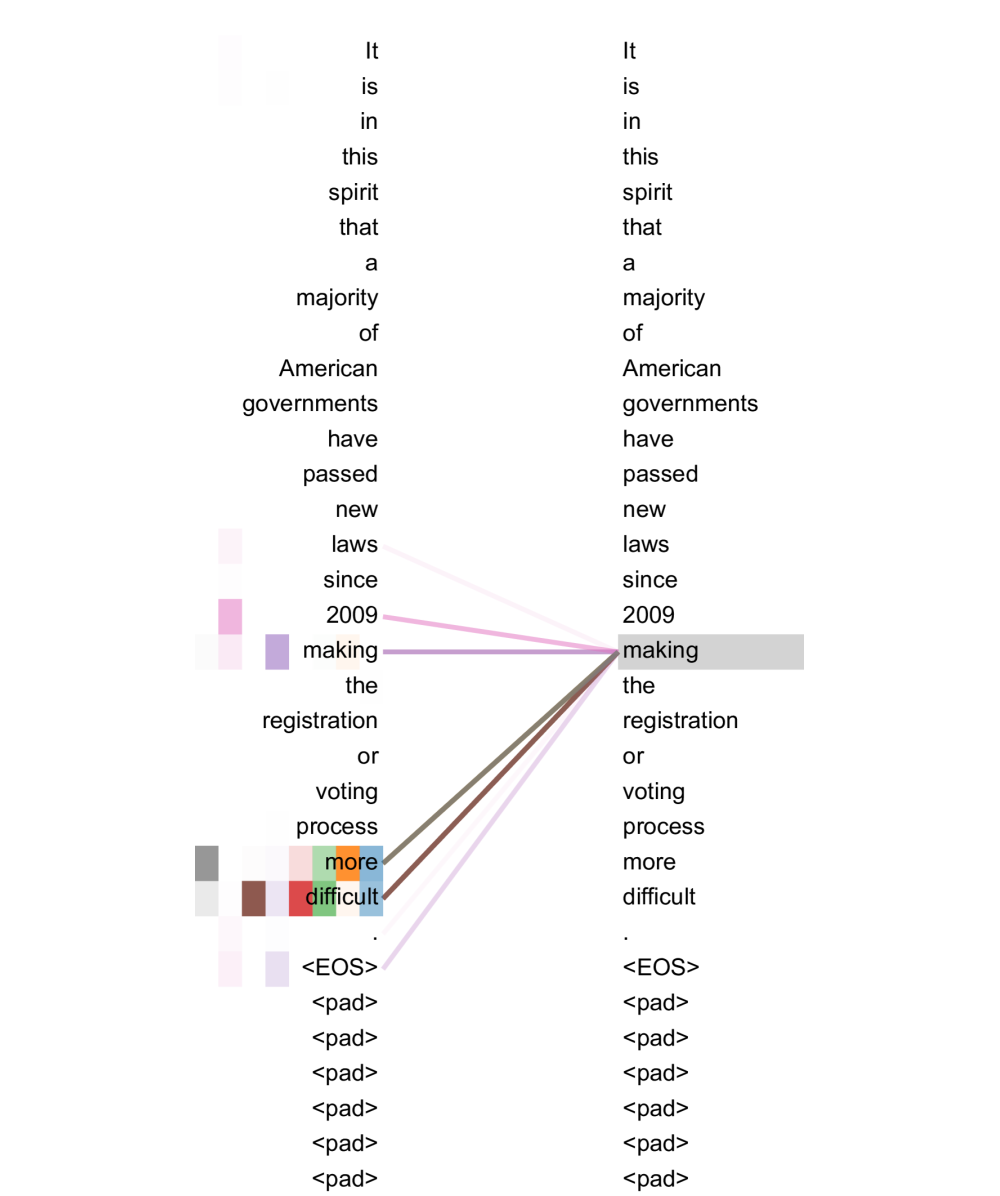
\includegraphics[width=\textwidth]{project/img/attention.png}
        \caption{Example of attention mechanism in the encoder. Taken from
        `Attention Is All You Need' \citep{attention}.}
        \label{attentionLinks}
    \end{minipage}
   \hspace{0.05\textwidth}
    \begin{minipage}{0.475\textwidth}
        \centering
        \chessboard[setfen=r3r1n1/bp6/p2p2kp/3N4/2P3n1/1PQ3Pq/P4P2/4RRK1 w - -
        0 1,
                    pgfstyle=border,markfields={d5},
                    pgfstyle=straightmove,
                    markmoves={f4-g6,f4-h3,c7-a8,c7-e8,d5-c7,d5-f4},
                    pgfstyle=color,opacity=0.5,
                    color=blue,markfields={f4,c7},
                    pgfstyle=color,opacity=0.5,
                    color=red,markfields={h3,g6,a8,e8}]
        \caption{Example of a relationship between chess pieces.}

        \label{chessPuzzleLinks}
    \end{minipage}
\end{figure}

\section{Data Preparation}

We formulate the problem of chess puzzle analysis as a multi-label
classification problem. Given a chess puzzle position in bitboard format,
i.e.\@ a $12\times8\times8$ binary tensor, we aim to predict a binary indicator
vector which encodes the labels of the puzzle themes. Slightly more formally,
the element $B[z, x, y]$ of bitboard $B$ is $1$ iff there is a piece $z \in
\{\texttt{p}, \texttt{P}, \texttt{n}, \texttt{N}, \texttt{b}, \texttt{B},
\texttt{r}, \texttt{R}, \texttt{q}, \texttt{Q}, \texttt{k},
\texttt{K}\}$\footnote{FEN-inspired -- white pieces are uppercase,
black pieces are lowercase.} at rank $x \in \{\texttt{1}, \texttt{2},
\texttt{3}, \texttt{4}, \texttt{5}, \texttt{6}, \texttt{7}, \texttt{8}\}$},
file $y \in \{\texttt{a}, \texttt{b}, \texttt{c}, \texttt{d}, \texttt{e},
\texttt{f}, \texttt{g}, \texttt{h}\}$.

Given a dataset with $N$ distinct puzzle labels ($N=60$ for the Lichess puzzle
database), we assign each label an index $i$ and form a binary $N$-dimensional
vector $x$ such that $x[i]=1$ iff the puzzle is labelled with that label. This
is a common technique to reduce a multi-label classification into a more
tractable problem.

To make learning easier (and to decrease implementation complexity), we
transform all chess positions to be from the perspective of White. This has
negligible additional overhead, as it requires a simple mirror and has great
benefits, as the model no longer needs to distinguish between white-to-move and
black-to-move puzzles.

\section{Model Architecture}

\begin{figure}[H]
        \centering
        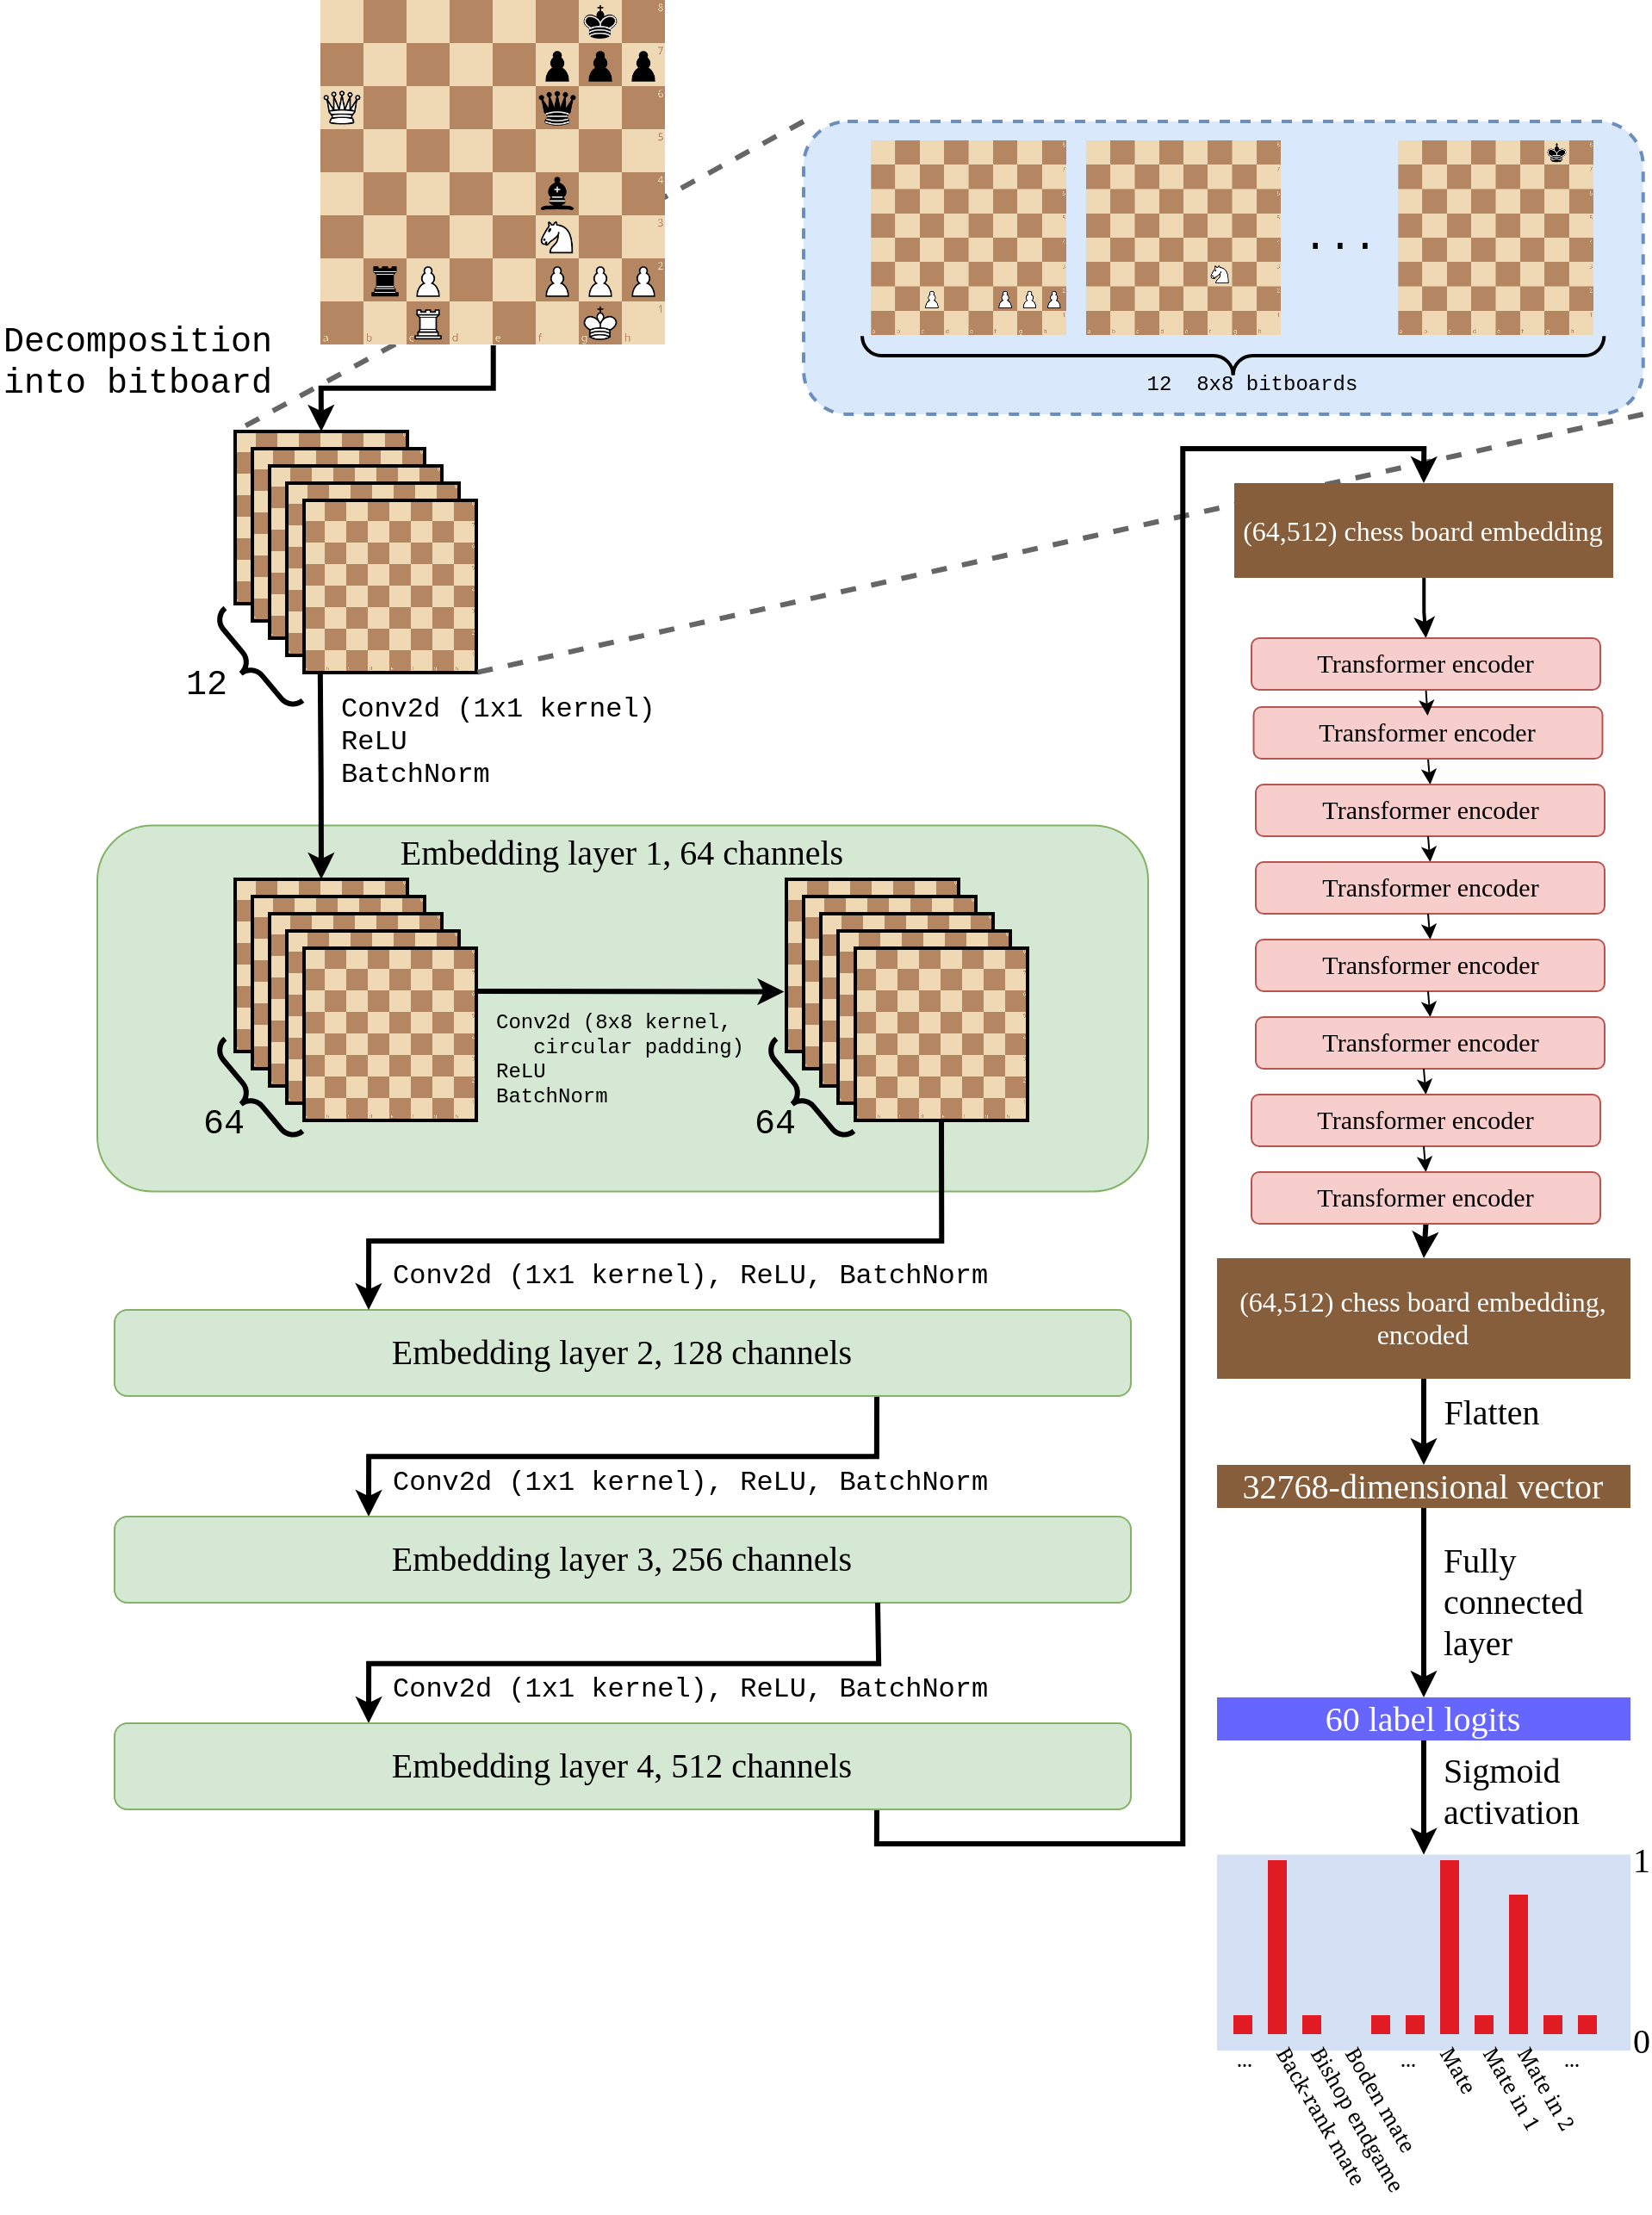
\includegraphics[width=\textwidth]{project/img/ml_diagram.png}
        \caption{High-level overview of the model architecture.}
        \label{MLDiagram}
\end{figure}






\chapter{The Tree-Based Approach}\label{treeChapter}

In this section, we propose a different novel approach to puzzle
classification, focusing on unsupervised puzzle clustering and defining a
distance function between various chess puzzles.

Section \ref{treeS1} gives a bird's eye view of the logic and design of the
algorithm. Subsection \ref{treeS11} introduces labelled search trees;
subsections \ref{treeS12}, \ref{treeS13} explain how to create them.

Section \ref{treeS2} looks at the outcomes of these trees, with subsection
\ref{treeS21} exploring how they can be used for finding similar chess
problems, and subsections \ref{treeS22}, \ref{treeS23} exploring unsupervised
puzzle clustering.

\section{Overview}\label{treeS1}

This method seeks to combine and build upon two approaches seen in the above
literature review: the tree-based puzzle difficulty classification
\citep{chessTrees} covered in Section \ref{chessTreesOverview} and chess
position similarity using dynamic features \citep{chessMotifs} covered in
Section \ref{chessMotifsOverview}. We hypothesise that by combining these
approaches to construct meaningful search trees with additional node labels,
defining a distance function for individual chess moves, and applying a
labelled tree edit distance function \citep{editDistTrees}, we would be able to
calculate `closeness' of chess puzzles. This could also help refine the work of
\citet{chessTrees} by finer segregating puzzles by difficulty level.

\subsection{Representing Puzzles With Labelled Trees}\label{treeS11}

As explored by \citet{chessTrees}, `meaningful search trees' have predictive
possibility of a puzzle's difficulty. These trees are constructed by analysing
powerful moves that either gain, or at least do not worsen a side's position. 

By additionally labelling these trees with move information, we hope to build
upon this work. To demonstrate the intuition behind this idea, there are two
labelled search trees shown in Figures \ref{tree1}, \ref{tree2}. These are the
search trees for positions in Figures \ref{chess5}, \ref{chess6} which feature
a identical and complex tactical motif. 

In the following trees, algebratic notation of the moves is shown, along with 4
slash-delimited integers, which correspond to: pieces attacked, pieces
defended, number of attackers, number of defenders.\footnote{As the moves must
be legal, this means a king move will never have any attackers, and any
check/mate will have at least 1 piece attacked -- the enemy king.} Whilst the 2
trees do not look similar visually (their size being the main problem), the
first 3 plies are very similar. 

\begin{figure}[H]
    \begin{minipage}{0.475\textwidth}
        \centering
        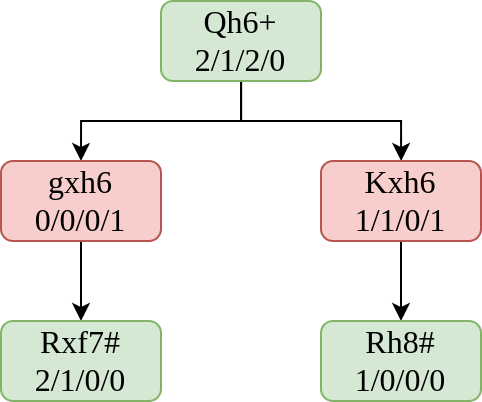
\includegraphics[width=\textwidth]{project/img/trees/1.drawio.png}
        \caption{Labelled search tree for game in \ref{chess5}}
        \label{tree1}
    \end{minipage}
    \hspace{0.05\textwidth}
    \begin{minipage}{0.475\textwidth}
        \centering
        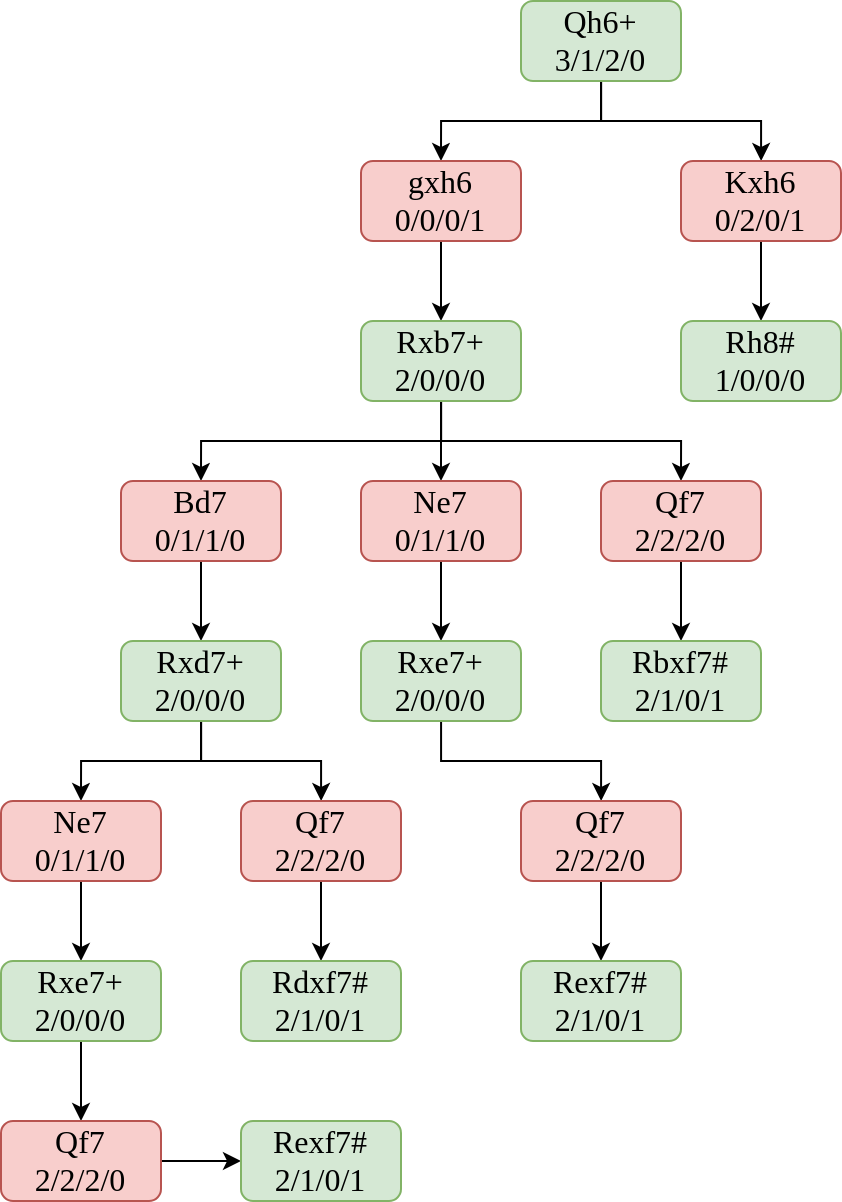
\includegraphics[width=\textwidth]{project/img/trees/2.drawio.png}
        \caption{Labelled search tree for game in \ref{chess6}}
        \label{tree2}
    \end{minipage}
\end{figure}

In Figures \ref{puzzle5}, \ref{puzzle6} are two chess puzzles from the paper
`Automatic Recognition of Similar Chess Motifs' \citep{chessMotifs}. Despite
their visual difference, these both feature a rook sacrifice, and an imminent
queen checkmate helped by the powerful light-squared bishop. This similarity is
not immediately obvious, but the search trees for these puzzles is almost
identical, except for minor attacker/defender discrepancies. The trees are
shown in Figures \ref{tree3}, \ref{tree4}. These puzzles were already
successfully grouped by \citet{chessMotifs}.

\begin{figure}[H]
    \begin{minipage}{0.475\textwidth}
        \centering
        \chessboard[setfen= 4r1k1/1b3pp1/4p3/p2r4/7R/2B1Q1PP/P1P1RP1K/1q6 w - -
        0 1]
        \caption{Taken from `Automatic Recognition of Similar Chess Motifs'
        \citep{chessMotifs}. White mates in 3 (\texttt{1.Rh8+ Kxh8 2.Qh6+ Kg8
        3.Qxg7#}).}
        \label{puzzle5}
    \end{minipage}
    \hspace{0.05\textwidth}
    \begin{minipage}{0.475\textwidth}
        \centering
        \chessboard[setfen=r5k1/5pp1/8/3p3R/2q4P/PbB2P2/1P1Q2P1/K7 w q - 0 1]
            \caption{Also taken from `Automatic Recognition of Similar Chess
            Motifs' \citep{chessMotifs}. White mates in 3 with the same moves
            as the puzzle on the left.}
        \label{puzzle6}
    \end{minipage}
\end{figure}

\begin{figure}[H]
    \begin{minipage}{0.475\textwidth}
        \centering
        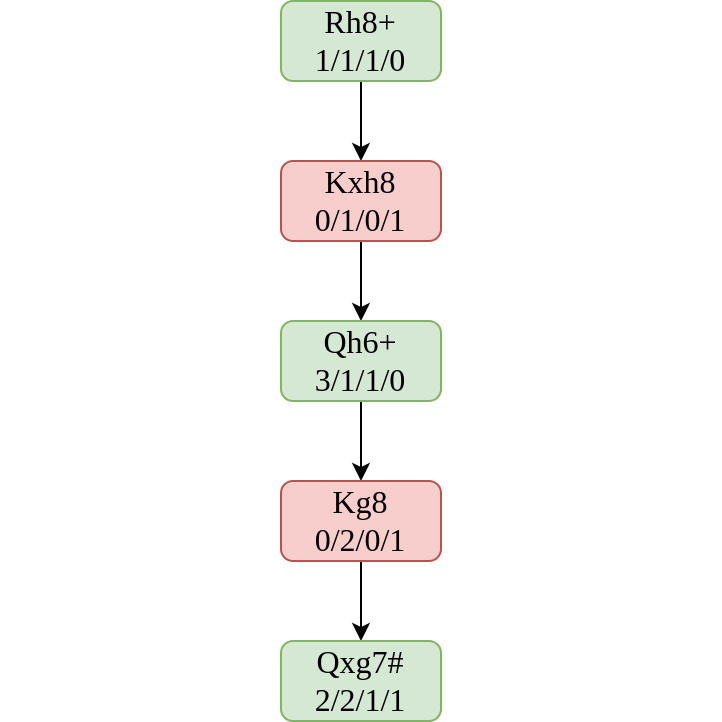
\includegraphics[width=\textwidth]{project/img/trees/3.drawio.png}
        \caption{Labelled search tree for game in Figure \ref{puzzle5}.}
        \label{tree3}
    \end{minipage}
    \hspace{0.05\textwidth}
    \begin{minipage}{0.475\textwidth}
        \centering
        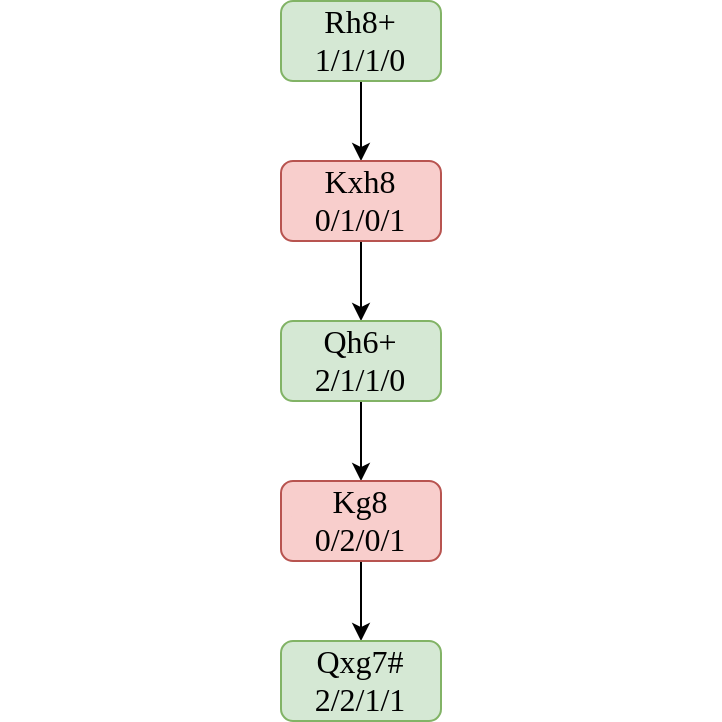
\includegraphics[width=\textwidth]{project/img/trees/4.drawio.png}
        \caption{Labelled search tree for game in Figure \ref{puzzle6}.}
        \label{tree4}
    \end{minipage}
\end{figure}

\subsection{Meaningful Tree Generation}\label{treeS12}

Similar to the work of \citet{chessTrees}, Stockfish (depth=20) was used to
generate meaningful trees of a maximum depth of 5 ply. Each level of the tree
has a maximum of 4 possible moves that are within 100 centipawns (arbitrarily
chosen) of the best move.

\citet{chessTrees} writes: ``[A high branching factor] means that the position
is already so strong that it no longer matters what move the player chooses
because almost everything wins.''; the tree search is terminated if the best 4
moves for the losing side are within 100 centipawns. While this differs from
the quote above, it causes trees to terminate when the puzzle is completed (any
move for the losing side is equally bad), as opposed to one move before (any
move for the winning side is equally good). Finally, a checkmate naturally
indicates that the puzzle is solved. 

This analysis is continued until either every branch of the puzzle is
exhausted, whether because it has solved the puzzle, or ran out of the maximum
depth of 5.

Whilst generating the tree nodes, each move is annotated with a list of
attributes describing the properties of these move. The exhaustive list of the
attributes we consider is as follows:

\begin{itemize}
    \item Colour of the piece
    \item Piece name (queen, rook, etc.\@)
    \item Depth of the node
    \item File, rank, diagonals (2 types: parallel to \texttt{a1-h8} or
        \texttt{a8-h1}) of the source square
    \item File, rank, diagonals of the target square
    \item Chebyshev distance (number of king moves) between source and target
        squares     
    \item Which piece is captured (if any)
    \item Delivers check or not
    \item Delivers mate or not
    \item Number of enemy pieces attacked after the move
    \item Number of friendly pieces defended after the move
    \item Number of enemy attackers after the move
    \item Number of friendly defenders after the move
\end{itemize}

In total, we generated 3.7 million game trees which took about 10000 hours of
CPU time. This was done with the help of the Department of Computing's HTCondor
cluster.

\subsection{What Makes Chess Moves Similar?}\label{treeS13}

Given the list in Section \ref{treeS12}, we define a distance function
between two given lists of attributes. All of the parameters are completely
arbitrary and were devised by an intermediate chess player. In Table
\ref{distanceTable}, the `penalties' for each discrepancy is listed. The final
distance between two nodes is the sum of all of the per-item distances.

The depth of the node affects the final scaling for the distance. The reasoning
behind this is that an initial move is much more important when comparing two
puzzles, but later moves are less important. This is also because there is
usually a lot of differences later in the move tree, and harshly penalising led
to worse results, from early experiments. The depth multipliers are: $4, 1,
0.5, 0.25, 0.1, 0.05$ for depths $0$ through to $5$, respectively.

\begin{table}[H]
  \centering
  \begin{tabular}{lrl}
      Condition & Penalty & Note \\
      \hline
      Different colour & $\infty$ & Implementation detail \\
      &&\\
      Pieces are queen/rook & $25$ & Heavy pieces are used similarly \\
      Pieces are queen/bishop& $50$ & Both can attack diagonally \\
      Pieces are different and not QR/QB& $100$ & \\
      &&\\
      Differing source rank/file/diagonal & $3$ each & \\
      Differing target rank/file/diagonal & $3$ each & \\
      Chebyshev distances $d_1, d_2$ & $|d_1-d_2|$ & Move distance is often
      not important \\
      &&\\
      Capture and non-capture & $50$ & \\
      Capture of different pieces & $10$ & \\
      Checking and non-checking & $25$ & \\
      Mate and non-mate & $50$ & \\
      &&\\
      Number of enemies attacked, $n_1, n_2$ & $3|n_1-n_2|$ & \\
      Number of allies defended, $n_1, n_2$ & $2|n_1-n_2|$ & \\
      Number of attackers, $n_1, n_2$ & $3|n_1-n_2|$ & \\
      Number of defenders, $n_1, n_2$ & $2|n_1-n_2|$ & \\
  \end{tabular}
  \caption{Breakdown of the node distance function for meaningful move trees}
  \label{distanceTable}
\end{table}

This distance function defines a distance between nodes of move trees. Together
with the unordered labelled tree edit distance algorithm \citep{editDistTrees},
we can now compare any two chess puzzles. As an example, Table
\ref{distanceComparisons} shows the distances between the puzzles in Figures
\ref{chess1}, \ref{chess2} (back-rank mate in 1), \ref{puzzle5}, \ref{puzzle6}
(rook sacrifice, mate in 3) and \ref{chess5}, \ref{chess6} (complex mating
sequence).

\begin{table}[H]
  \centering
  \begin{tabular}{r|cccccc}
    Figure &
    \ref{chess1}&\ref{chess2}&\ref{puzzle5}&\ref{puzzle6}&\ref{chess5}&\ref{chess6}
    \\
    \hline
    \ref{chess1} & $0$ & $232$ & $978.5$ & $982.5$ & $1422$ & $1714$ \\ 
    \ref{chess2} & $232$ & $0$ & $1086.5$ & $1082.5$ & $1278$ & $1586$ \\
    \ref{puzzle5} & $978.5$ & $1086.5$ & $0$ & $46.5$ & $789$ & $1033.15$ \\
    \ref{puzzle6} & $982.5$ & $1082.5$ & $46.5$ & $0$ & $795$ & $1035.15$ \\
    \ref{chess5} & $1422$ & $1278$ & $789$ & $795$ & $0$ & $417$ \\
    \ref{chess6} & $1714$ & $1586$ & $1033.15$ & $1035.15$ & $417$ & $0$ \\
  \end{tabular}
  \caption{Distance matrix for a few chess puzzles.}
  \label{distanceComparisons}
\end{table}

\section{Applications}\label{treeS2}

\subsection{Finding Similar Positions Given a Puzzle}\label{treeS21}

Generating the distance matrix in Table \ref{distanceComparisons} is
prohibitively expensive, as it scales quadratically with the number of
positions -- calculating this for the whole Lichess database is difficult. By
extracting one row, however, we can rank puzzles in order of similarity to a
given puzzle.

For a simple back-rank mate in 1 puzzle, this is incredibly effective. Given
the puzzle in Figure \ref{chess1}, we are able to find positions like the ones
in Figures \ref{m11} and \ref{m22}. These positions are arguably more complex
as there are more pieces on the board, making it harder to find the winning
move.

\begin{figure}[H]
    \begin{minipage}{0.475\textwidth}
        \centering
        \chessboard[setfen= 6k1/pr4pR/2p2pP1/2Pp4/5N2/P1r2P2/3RP3/3K4 b - - 1
        28]
        \caption{Distance $40$ to Figure \ref{chess1}. Solution:
        \texttt{1...Rb1\#}}
        \label{m11}
    \end{minipage}
    \hspace{0.05\textwidth}
    \begin{minipage}{0.475\textwidth}
        \centering
        \chessboard[setfen=1r4k1/6p1/p1R1p2p/8/P6P/3R4/2P2rP1/3K4 b - - 0 30]
        \caption{Distance $0$ to Figure \ref{chess1}. Solution:
        \texttt{1...Rb1\#}}
        \label{m22}
    \end{minipage}
\end{figure}

With a more complex position, such as the mate in two in Figure \ref{chess5},
this method returns the positions in Figures \ref{mag1} and \ref{mag2}. These
do not feature exactly the same tactic, but they are nonetheless similar,
featuring a rook sacrifice on \texttt{h3} and different mating squares
depending on White's response.

\begin{figure}[H]
    \begin{minipage}{0.475\textwidth}
        \centering
        \chessboard[setfen=2k3r1/p1p4p/8/pP1QR3/P2P3P/2P3r1/5RPK/3q4 b - - 2 30]
        \caption{Distance $255$ to Figure \ref{chess5}. Solution:
        \texttt{1...Rh3+ (2.Kxh3 Qh1\#) (2.gxh3 Qg1\#)}}
        \label{mag1}
    \end{minipage}
    \hspace{0.05\textwidth}
    \begin{minipage}{0.475\textwidth}
        \centering
        \chessboard[setfen=6rk/pR6/2p4p/8/4PP2/P2P2r1/P2Q1RPK/q7 b - - 4 35]
        \caption{Distance $259$ to Figure \ref{chess5}. Solution identical to
        puzzle on the left.}
        \label{mag2}
    \end{minipage}
\end{figure}

\subsection{Unsupervised Clustering on Puzzle Distances}\label{treeS22}

To take this further, a distance matrix was constructed for a random sample of
10000 puzzles from the Lichess puzzle database. A few labelled puzzles were
added to help with analysis of the results. A selection of unsupervised
clustering algorithms were ran on this matrix to identify clusters of puzzles
which are all similar to each other. Many of the standard clustering algorithms
were not available due to the nature of the problem -- there is no obvious
vector space representing the search trees, ruling out algorithms like K-means
\citep{lloyd1982least} or Mean Shift \citep{fukunaga1975estimation}.

We attempted Agglomerative Clustering (average, single, complete)
\citep{szekely2005hierarchical}, DBSCAN \citep{dbscan}, and HDBSCAN
\citep{hdbscan} on this subset of the database. The results are shown in Tables
\ref{tabAC}, \ref{tabDBSCAN} and \ref{tabHDBSCAN}. Visualisations of the
highlighted rows can be seen in Section \ref{treeS23}.

\begin{table}[H]
  \centering
  \begin{adjustbox}{width=\textwidth}
  \begin{tabular}{lr|rccccrrrrrrr}
    \multicolumn{2}{l}{Parameters}&&\multicolumn{4}{c}{Puzzle is in a cluster}
    &&
    \multicolumn{6}{c}{Cluster size statistics} \\

    Linkage&Distance threshold&Number of clusters&\rotatebox{90}{Backrank M1} &
    \rotatebox{90}{Knight fork} & \rotatebox{90}{Greek gift} &
    \rotatebox{90}{Rook sac M3} & Outlier \% & \rotatebox{90}{Mean} &
    \rotatebox{90}{Min} & \rotatebox{90}{Q1} & \rotatebox{90}{Median} &
    \rotatebox{90}{Q3} & \rotatebox{90}{Max} \\

    \hline
    average&100&17040&Y&Y&Y&Y&0.0&1.17&1&1&1&1&178\\
    average&250&13812&Y&Y&Y&Y&0.0&1.45&1&1&1&1&1000\\
    average&500&8600&Y&Y&Y&Y&0.0&2.33&1&1&1&1&1863\\
    average&750&2759&Y&Y&Y&Y&0.0&7.25&1&1&1&2&2879\\
    average&1000&687&Y&Y&Y&Y&0.0&29.12&1&1&2&4&4069\\
    complete&100&17263&Y&Y&Y&Y&0.0&1.16&1&1&1&1&85\\
    complete&250&14064&Y&Y&Y&Y&0.0&1.42&1&1&1&1&611\\
    complete&500&9197&Y&Y&Y&Y&0.0&2.18&1&1&1&1&1000\\
    complete&750&3826&Y&Y&Y&Y&0.0&5.23&1&1&1&4&1780\\
    complete&1000&1404&Y&Y&Y&Y&0.0&14.25&1&2&3&8&2039\\
    single&100&16809&Y&Y&Y&Y&0.0&1.19&1&1&1&1&611\\
    single&250&13513&Y&Y&Y&Y&0.0&1.48&1&1&1&1&2642\\
    \rowcolor{lightgray} single&500&7418&Y&Y&Y&Y&0.0&2.7&1&1&1&1&9888\\
    single&750&1743&Y&Y&Y&Y&0.0&11.48&1&1&1&1&16224\\
    single&1000&231&Y&Y&Y&Y&0.0&86.6&1&1&1&1&19774\\


  \end{tabular}
  \end{adjustbox}
  \caption{Results of Agglomerative Clustering}
  \label{tabAC}
\end{table}

\begin{table}[H]
  \centering
  \begin{adjustbox}{width=\textwidth}
  \begin{tabular}{rr|rccccrrrrrrr}
    \multicolumn{2}{l}{Parameters}&&\multicolumn{4}{c}{Puzzle is in a cluster}
    &&
    \multicolumn{6}{c}{Cluster size statistics} \\

    Epsilon&Minimum samples&Number of clusters&\rotatebox{90}{Backrank M1} &
    \rotatebox{90}{Knight fork} & \rotatebox{90}{Greek gift} &
    \rotatebox{90}{Rook sac M3} & Outlier \% & \rotatebox{90}{Mean} &
    \rotatebox{90}{Min} & \rotatebox{90}{Q1} & \rotatebox{90}{Median} &
    \rotatebox{90}{Q3} & \rotatebox{90}{Max} \\

    \hline
    50&3&45&&&&&93.28&29.82&7&9&13&28&365\\
    50&5&45&&&&&93.28&29.82&7&9&13&28&365\\
    50&7&45&&&&&93.28&29.82&7&9&13&28&365\\
    50&9&37&&&&&93.65&34.32&9&10&16&28&365\\
    100&3&43&Y&&&Y&83.69&75.86&7&11&21&41&1000\\
    100&5&43&Y&&&Y&83.69&75.86&7&11&21&41&1000\\
    100&7&43&Y&&&Y&83.69&75.86&7&11&21&41&1000\\
    100&9&38&Y&&&Y&83.88&84.84&9&13&26&51&1000\\
    250&3&36&Y&&Y&Y&67.36&181.39&7&9&25&87&2643\\
    250&5&36&Y&&Y&Y&67.36&181.39&7&9&25&87&2643\\
    250&7&36&Y&&Y&Y&67.36&181.39&7&9&25&87&2643\\
    250&9&32&Y&&Y&Y&67.60&202.56&9&13&30&112&2643\\
    500&3&5&Y&Y&Y&Y&37.03&2519.4&17&256&391&2039&9894\\
    500&5&5&Y&Y&Y&Y&37.03&2519.4&17&256&391&2039&9894\\
    \rowcolor{lightgray} 500&7&5&Y&Y&Y&Y&37.03&2519.4&17&256&391&2039&9894\\
    500&9&5&Y&Y&Y&Y&37.03&2519.4&17&256&391&2039&9894\\
    750&3&2&Y&Y&Y&Y&8.69&9133.0&2039&5586&9133&12680&16227\\
    750&5&2&Y&Y&Y&Y&8.69&9133.0&2039&5586&9133&12680&16227\\
    750&7&2&Y&Y&Y&Y&8.69&9133.0&2039&5586&9133&12680&16227\\
    750&9&2&Y&Y&Y&Y&8.69&9133.0&2039&5586&9133&12680&16227& \\

  \end{tabular}
  \end{adjustbox}
  \caption{Results of DBSCAN}
  \label{tabDBSCAN}
\end{table}

\begin{table}[H]
  \centering
  \begin{adjustbox}{width=\textwidth}
  \begin{tabular}{rr|rccccrrrrrrr}
    \multicolumn{2}{l}{Parameters}&&\multicolumn{4}{c}{Puzzle is in a cluster}
    &&
    \multicolumn{6}{c}{Cluster size statistics} \\

    Cluster selection $\epsilon$&Min cluster size&Number of
    clusters&\rotatebox{90}{Backrank M1} &
    \rotatebox{90}{Knight fork} & \rotatebox{90}{Greek gift} &
    \rotatebox{90}{Rook sac M3} & Outlier \% & \rotatebox{90}{Mean} &
    \rotatebox{90}{Min} & \rotatebox{90}{Q1} & \rotatebox{90}{Median} &
    \rotatebox{90}{Q3} & \rotatebox{90}{Max} \\

    \hline

    0&3&1347&Y&Y&&Y&42.57&8.53&3&3&5&9&338\\
    0&5&801&Y&Y&&Y&49.21&12.69&5&6&8&12&347\\
    0&7&546&Y&Y&&Y&52.17&17.52&7&8&10&15&917\\
    0&9&342&&Y&Y&Y&59.84&23.49&9&11&14&19&386\\
    25&3&1156&&Y&Y&Y&44.91&9.53&3&4&5&10&355\\
    25&5&693&Y&Y&Y&Y&49.6&14.55&5&6&8&13&352\\
    25&7&462&Y&Y&Y&Y&53.16&20.27&7&8&11&16&980\\
    25&9&354&&Y&Y&Y&58.77&23.3&9&10&13&20&383\\
    50&3&1212&&Y&Y&Y&42.80&9.44&3&3&5&9&353\\
    50&5&706&&Y&Y&Y&48.61&14.56&5&6&8&12&384\\
    50&7&479&Y&Y&Y&Y&50.94&20.48&7&8&10&15&901\\
    50&9&330&Y&Y&Y&Y&59.0&24.85&9&10&13&20&379\\
    100&3&1123&Y&Y&Y&Y&41.14&10.49&3&3&5&8&1000\\
    100&5&624&Y&Y&Y&Y&46.9&17.02&5&6&8&11&1000\\
    \rowcolor{lightgray}100&7&410&Y&Y&Y&Y&51.72&23.55&7&8&10&15&1000\\
    100&9&276&Y&Y&Y&Y&55.06&32.57&9&10&13&19&1000\\
    250&3&928&Y&Y&Y&Y&33.90&14.25&3&3&5&8&2606\\
    250&5&541&Y&Y&Y&Y&37.46&23.13&5&6&8&11&2853\\
    250&7&355&Y&Y&Y&Y&41.18&33.15&7&8&9&14&2853\\
    250&9&226&Y&Y&Y&Y&43.72&49.82&9&10&12&17&2611\\


  \end{tabular}
  \end{adjustbox}
  \caption{Results of HDBSCAN}
  \label{tabHDBSCAN}
\end{table}

From these tables, it is easy to identify the methods that really struggle to
create meaningful clusters out of the given chess puzzles. Namely, all variants
of Agglomerative Clustering produced results with either too many clusters
(10000+) of 1 puzzle each, or a megacluster consisting almost of the entire
subset of the database.. It is not obvious what an appropriate cluster count
result is; the Lichess database has approximately 60 unique themes, which gives
a very rough target. However, the Lichess database themes are not mutually
exclusive, unlike the cluster membership produced by these algorithms. 

A different heuristic used as a sign that a method is inappropriate is whether
it assigns a cluster to 4 simple chess puzzles. These are shown below. These
puzzles were selected as their tactical pattern is relatively common,
especially Figures \ref{chess11} and \ref{chess12}. This means that a
clustering method that fails to assign these a cluster (labelling them an
`outlier') is unlikely to be effective overall.

\begin{figure}[H]
    \begin{minipage}{0.475\textwidth}
        \centering
        \chessboard[setfen=6k1/5ppp/8/8/8/8/r4PPP/1R4K1 w - - 0 1]
        \caption{Backrank M1: \texttt{1.Rb8\#}}
        \label{chess11}
    \end{minipage}
    \hspace{0.05\textwidth}
    \begin{minipage}{0.475\textwidth}
        \centering
        \chessboard[setfen=8/1N6/1K6/4k1p1/2P1Pp1p/4n2P/3R2P1/8 b - - 0 49]
        \caption{Knight forks rook and king with \texttt{1...Nxc4+}}
        \label{chess12}
    \end{minipage}
\end{figure}


\begin{figure}[H]
    \begin{minipage}{0.475\textwidth}
        \centering
        \chessboard[setfen=
        r1bq1rk1/pp2nppp/1bn1p3/1N1pP3/1P6/P2B1N2/2P2PPP/R1BQK2R w KQ - 3 11]
        \caption{Greek gift sacrifice: \texttt{1.Bxh7+ Kxh7 2.Ng5+}}
        \label{chess13}
    \end{minipage}
    \hspace{0.05\textwidth}
    \begin{minipage}{0.475\textwidth}
        \centering
        \chessboard[setfen= 4r1k1/1b3pp1/4p3/p2r4/7R/2B1Q1PP/P1P1RP1K/1q6 w - -
        0 1]
        \caption{Rook sacrificed for mate in three: \texttt{1.Rh8+ Kxh8 2.Qh6+
        Kg8 3.Qxg7\#}}
        \label{chess14}
    \end{minipage}
\end{figure}

This allowed some parameter combinations of DBSCAN to be disqualified,
specifically the lower epsilon ones. Epsilon is the distance at which points
are considered to be in one neighbourhood \citep{dbscan}, and setting this too
low means similar puzzles are not given the same cluster. The distance matrix
in Table \ref{distanceComparisons} shows that puzzles which are similar to a
human can have a distance of 417, and this is by no means an upper limit.

Another interesting result is the percentage of outliers -- puzzles which have
so little neighbours around them that they are not given a cluster and
considered noise. This number hovers at around 50\% for HDBSCAN (Table
\ref{tabHDBSCAN}), and drops to about 8-9\% for DBSCAN (Table \ref{tabDBSCAN}).
Unfortunately, the lowest percentage happens when DBSCAN identifies 2 clusters,
which is far too few to draw meaningful conclusions from.

\subsection{Visualisations of Puzzle Clusters}\label{treeS23}

To illustrate what these clusters look like, we use t-distributed Stochastic
Neighbor Embedding (t-SNE), a method to visualise high dimensional data in two
or three dimensions, developed by \citet{tsne}. It should be noted that these
visualisations can be quite misleading \citep{wattenberg2016how}, but they are
nonetheless helpful for developing some sense of the structure and clustering.

In the following diagrams, vibrant points denote the clusters of the puzzles
above. Faintly coloured crosses are clusters which do not contain any of those
puzzles. Faintly coloured black points are outliers.

Figure \ref{tsne1} shows a t-SNE visualisation of the low-performing
Agglomerative Clustering. There are no outliers in this method, and every
puzzle is part of a cluster, causing multicoloured blobs. The biggest cluster,
containing just over half of the puzzles, is the cyan one, spanning multiple
t-SNE blobs. This megacluster contains all but one of the puzzles: the
back-rank mate in one in Figure \ref{chess11}. This visualisation clearly shows
that this method is not applicable.

\begin{figure}[H]
  \centering
  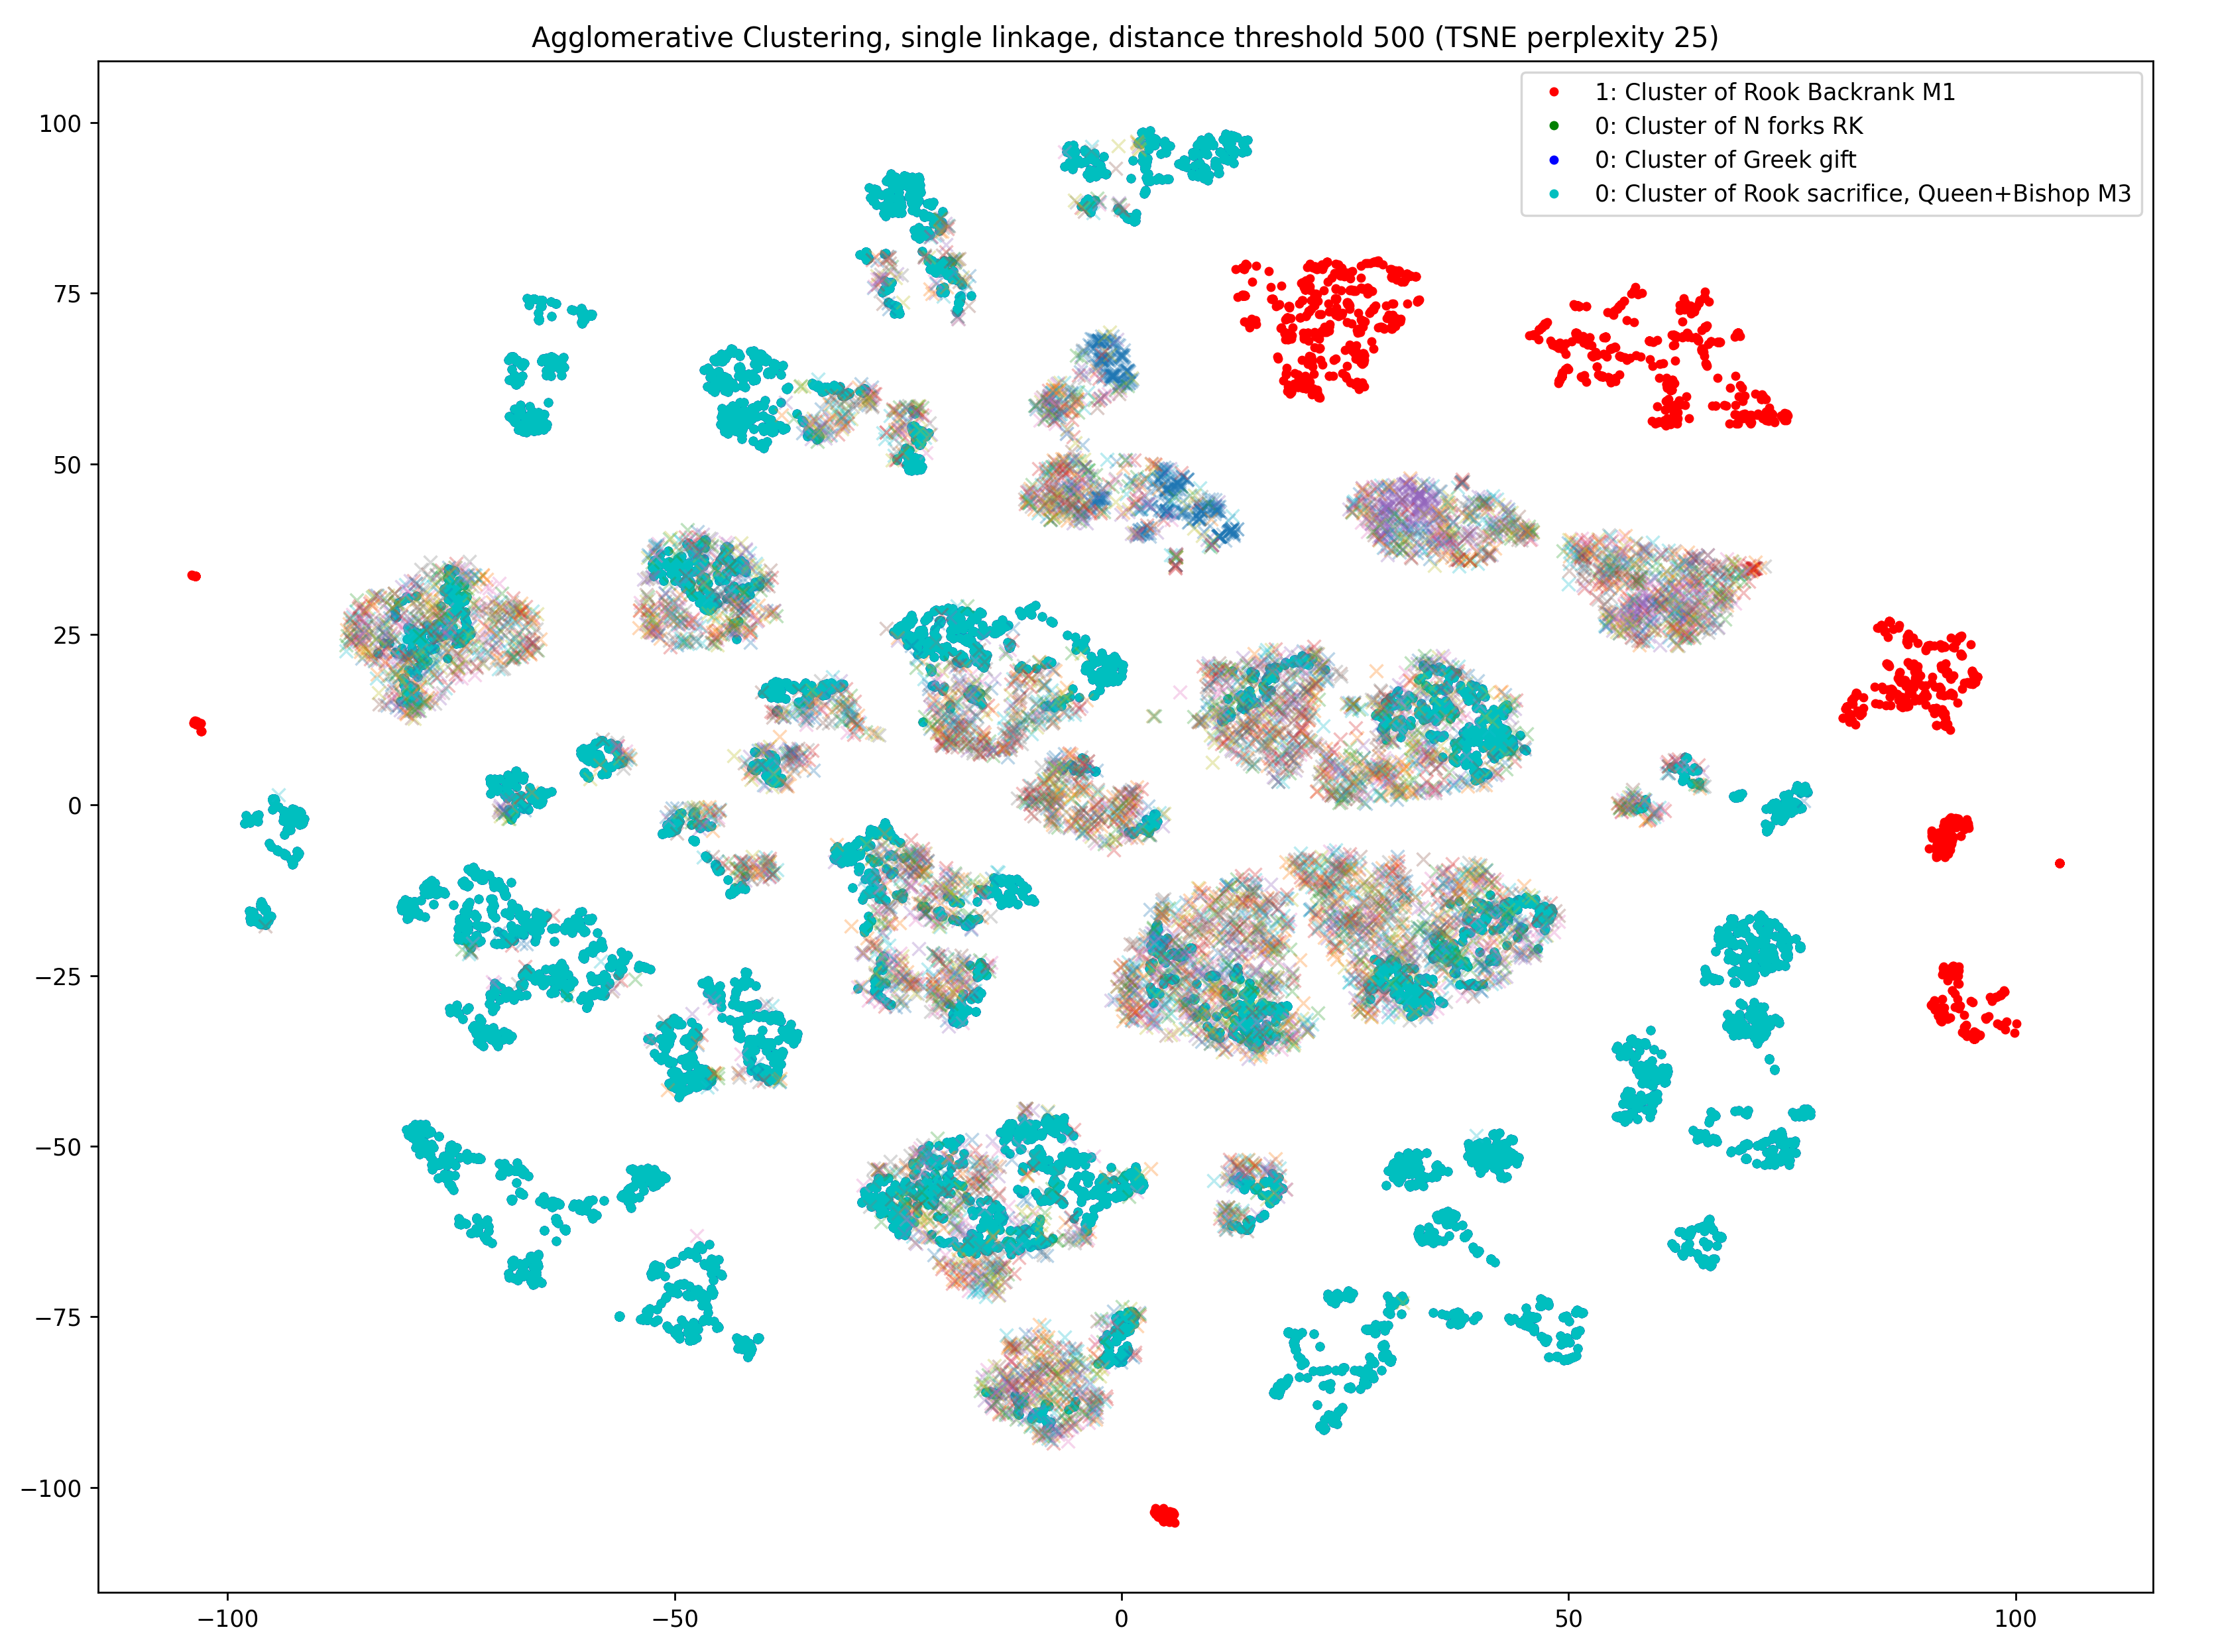
\includegraphics[width=\textwidth]{project/img/tsne/ac_25.png}
  \caption{Agglomerative Clustering (single linkage, distance threshold $500$)}
  \label{tsne1}
\end{figure}

A similar behaviour is seen with some of the DBSCAN attempts. Figure
\ref{tsne2} shows one of these, and whilst this also creates a megacluster, it
marks many puzzles as outliers. This method creates only 6 clusters, and we can
see the big orange and blue clusters in-between the red and cyan.

\begin{figure}[H]
  \centering
  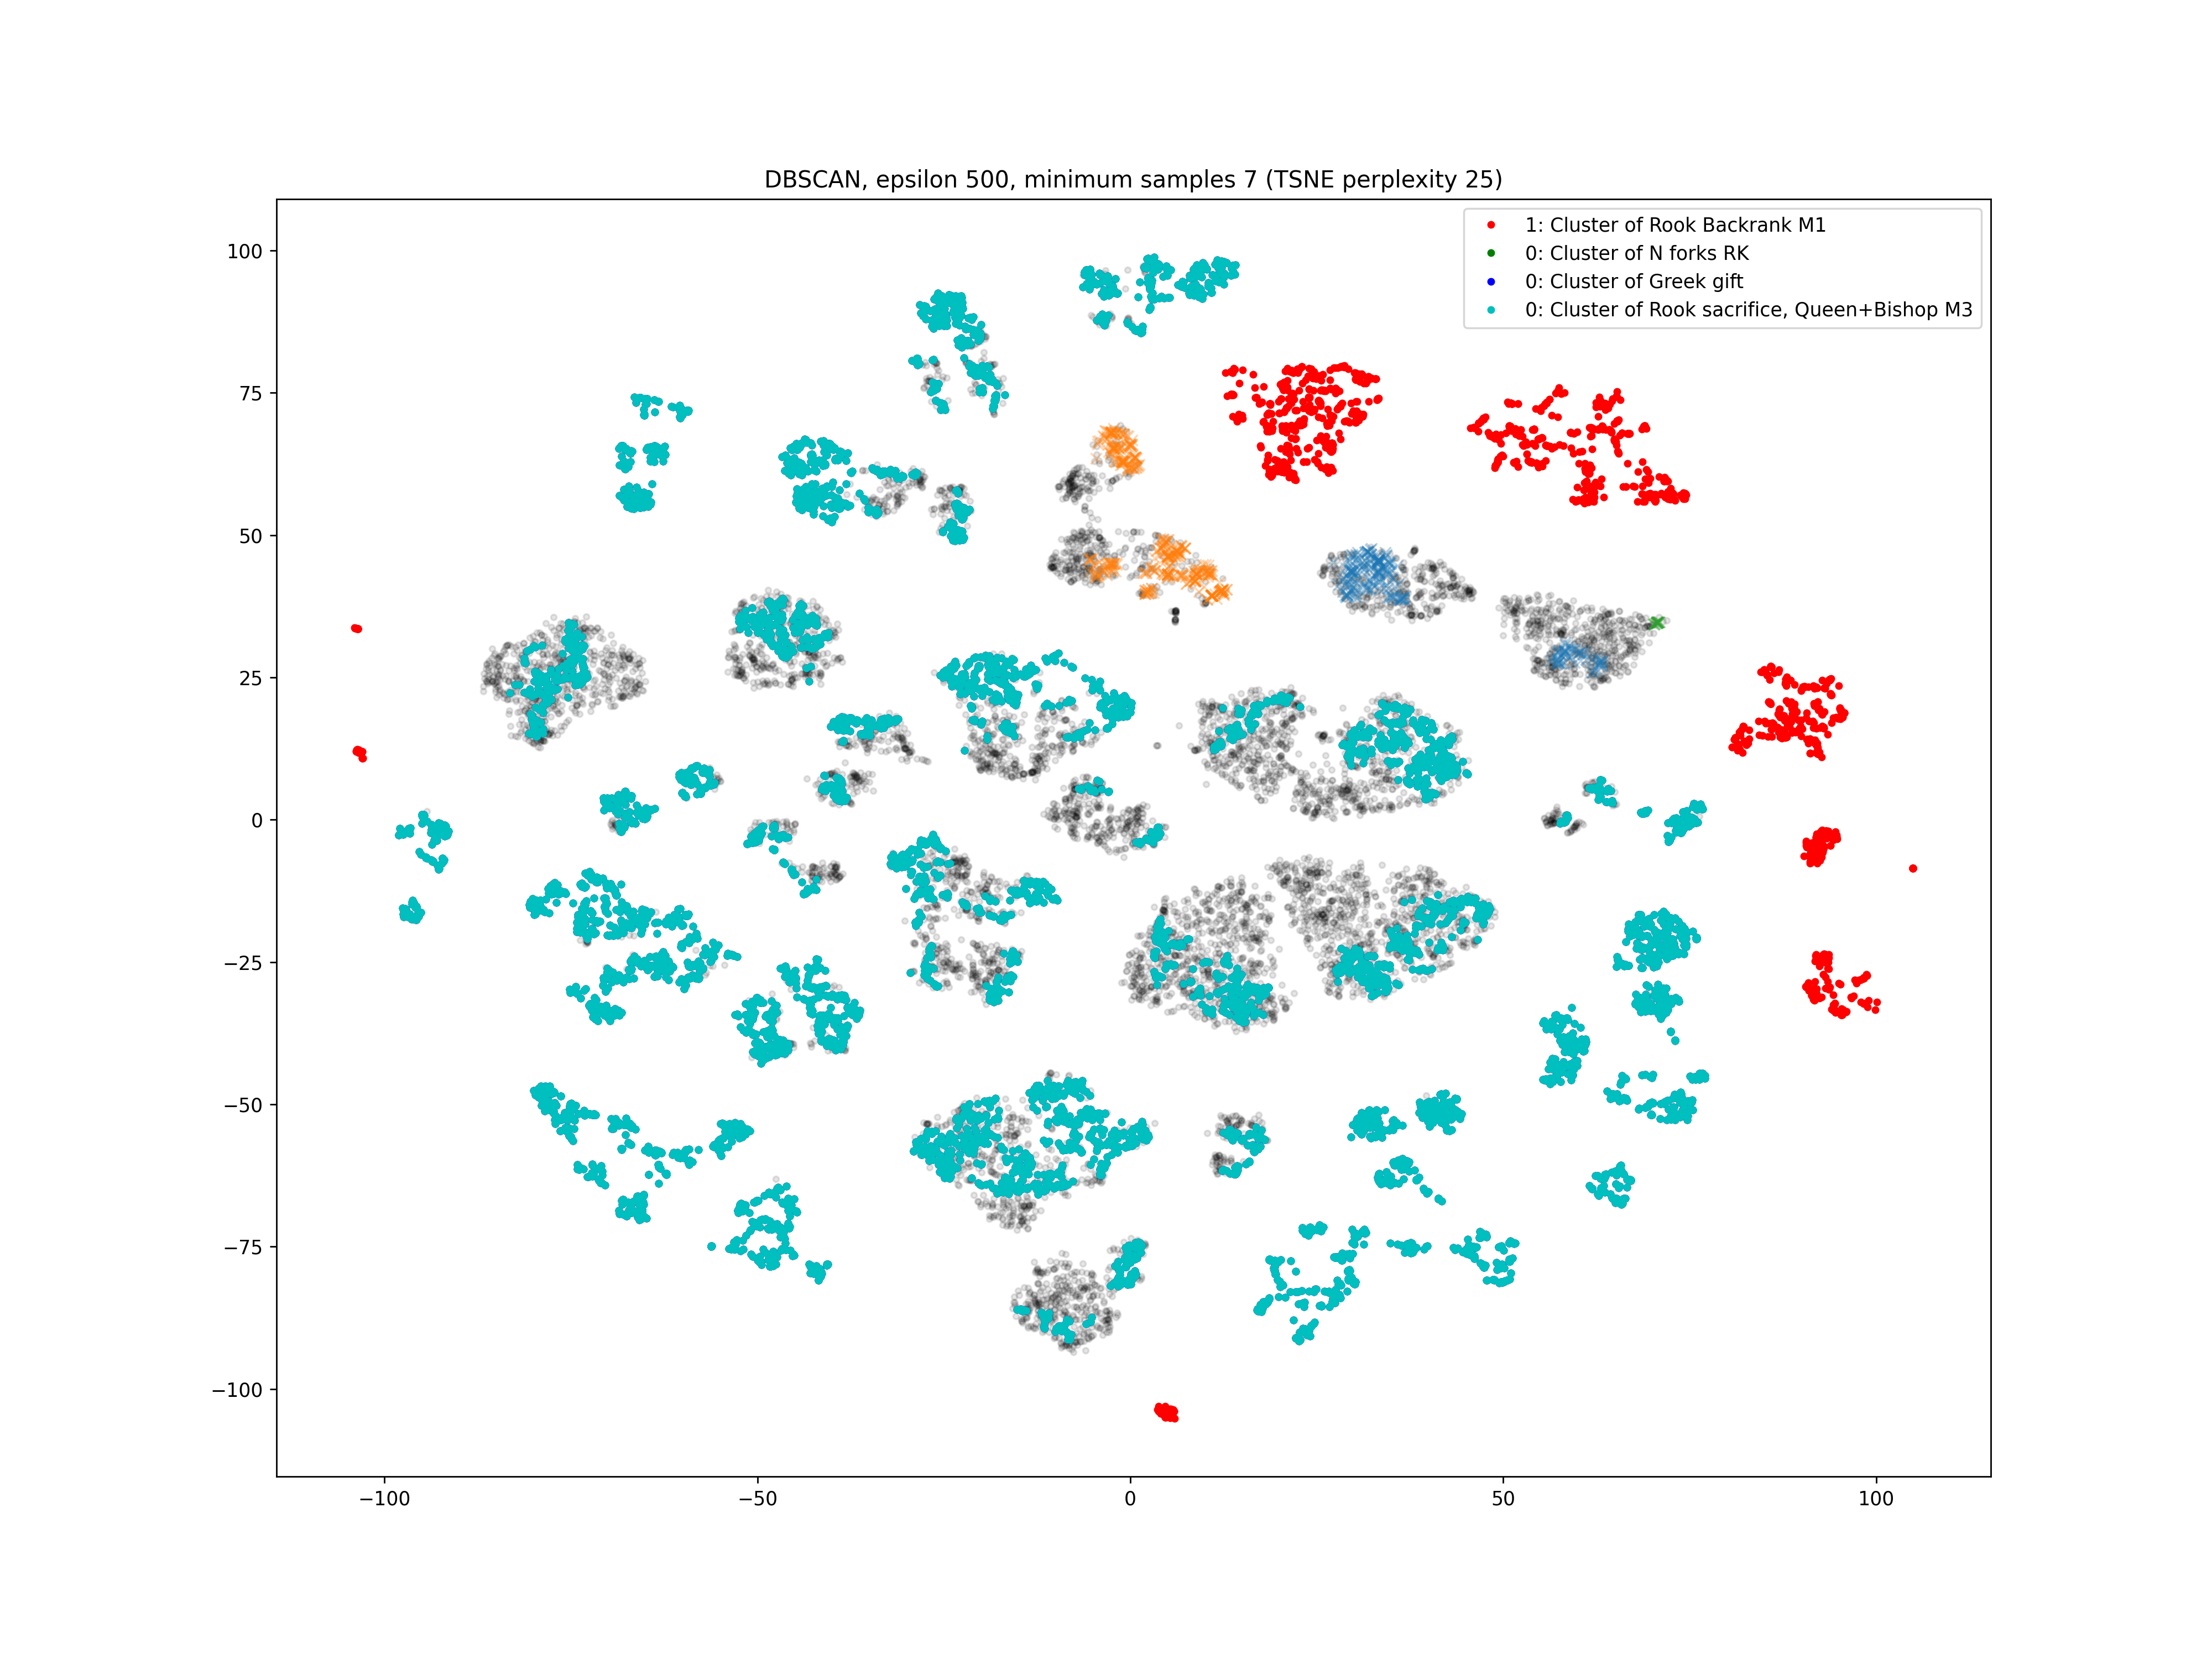
\includegraphics[width=\textwidth]{project/img/tsne/dbscan_500_25.png}
  \caption{DBSCAN, $\epsilon=500$, minimum samples $7$.}
  \label{tsne2}
\end{figure}

Taking samples from cluster 1 reveals that this method likely grouped all mate
in 1 puzzles into one cluster. Along with the puzzle in Figure \ref{chess11},
this cluster contains the puzzles in Figures \ref{dbscanCluster11} and
\ref{dbscanCluster12}. 

A more interesting result lies in sampling puzzles from a different cluster,
which does not feature any of the known puzzles. One such cluster, as
identified by DBSCAN, appears to capture endgames. Out of its 415 puzzles, 413
(99.5\%) are tagged on Lichess as `endgame', 196 (47.2\%) as `pawn endgame',
and 102 (24.6\%) as either `rook endgame', `knight endgame', or `bishop
endgame'. Figures \ref{dbscanCluster13} and \ref{dbscanCluster14} show some of
the example puzzles in this cluster.

This is already a promising result, but since the clustering is so coarse, it
is no surprise that one of them captures the broad theme of endgames. Luckily,
this is solved with HDBSCAN.

\begin{figure}[H]
    \begin{minipage}{0.475\textwidth}
        \centering
        \chessboard[setfen= 2rr2k1/ppb3pp/8/3p1q2/1P1Qn2P/P2KP2p/1B6/2RR4 w - -
        2 32]
        \caption{Puzzle sharing the cluster with Figure \ref{chess11}. Solution:
        \texttt{1.Qxg7\#}}
        \label{dbscanCluster11}
    \end{minipage}
    \hspace{0.05\textwidth}
    \begin{minipage}{0.475\textwidth}
        \centering
        \chessboard[setfen= r3k2r/pp1qbppp/2pp1n2/8/3QP3/2N2P1P/PPP2P2/R1B3RK b
        kq - 4 13]
        \caption{Same cluster as Figure \ref{chess11}. Solution:
        \texttt{1...Qxh3\#}}
        \label{dbscanCluster12}
    \end{minipage}
\end{figure}

\begin{figure}[H]
    \begin{minipage}{0.475\textwidth}
        \centering
        \chessboard[setfen=8/8/1p3k2/p6p/P3K1pP/1P4P1/8/8 w - - 5 46]
        \caption{Puzzle from the endgame cluster. Both sides' pawns are frozen,
        and White wins with \texttt{1.Kf4}, shouldering the black king away
        from the \texttt{h5} pawn.}
        \label{dbscanCluster13}
    \end{minipage}
    \hspace{0.05\textwidth}
    \begin{minipage}{0.475\textwidth}
        \centering
        \chessboard[setfen=5k2/1N3ppp/n3p3/P7/5P2/6P1/7P/6K1 b - - 0 33]
        \caption{Puzzle from the endgame cluster. \texttt{1...Ke7} traps the
        knight(!), which is lost a few moves later.}
        \label{dbscanCluster14}
    \end{minipage}
\end{figure}

Figure \ref{tsne3} shows HDBSCAN puzzle clustering. The megacluster which was
apparent in the previous two examples has been broken up, and there are a few
promising clusters. In total, there are 420 clusters, with a mean cluster size
of $22.82$. Unfortunately, the Greek gift puzzle (Figure \ref{chess13}) is
outside of any clusters, which is surprising, given the apparent effectiveness
of this algorithm.

Despite this, the clustering seems to perform much better than the former
attempts, and yields useful results. Cluster 333, under which the knight fork
puzzle (Figure \ref{chess12}) falls, contains 18 puzzles, of which 17 are
tagged with `short' and 15 with `fork'. Figures \ref{hCl1} and \ref{hCl2} are
examples from this cluster. Interestingly, the puzzle in Figure \ref{hCl2} is
not tagged as a `fork' , even though it undeniably forks the king and bishop.
The remaining puzzles with no `fork' tag in this cluster have been manually
checked and are indeed knight forks. This is a good result, as it shows that
this method can pick up on themes that the Lichess puzzle database missed.

\begin{figure}[H]
  \centering
  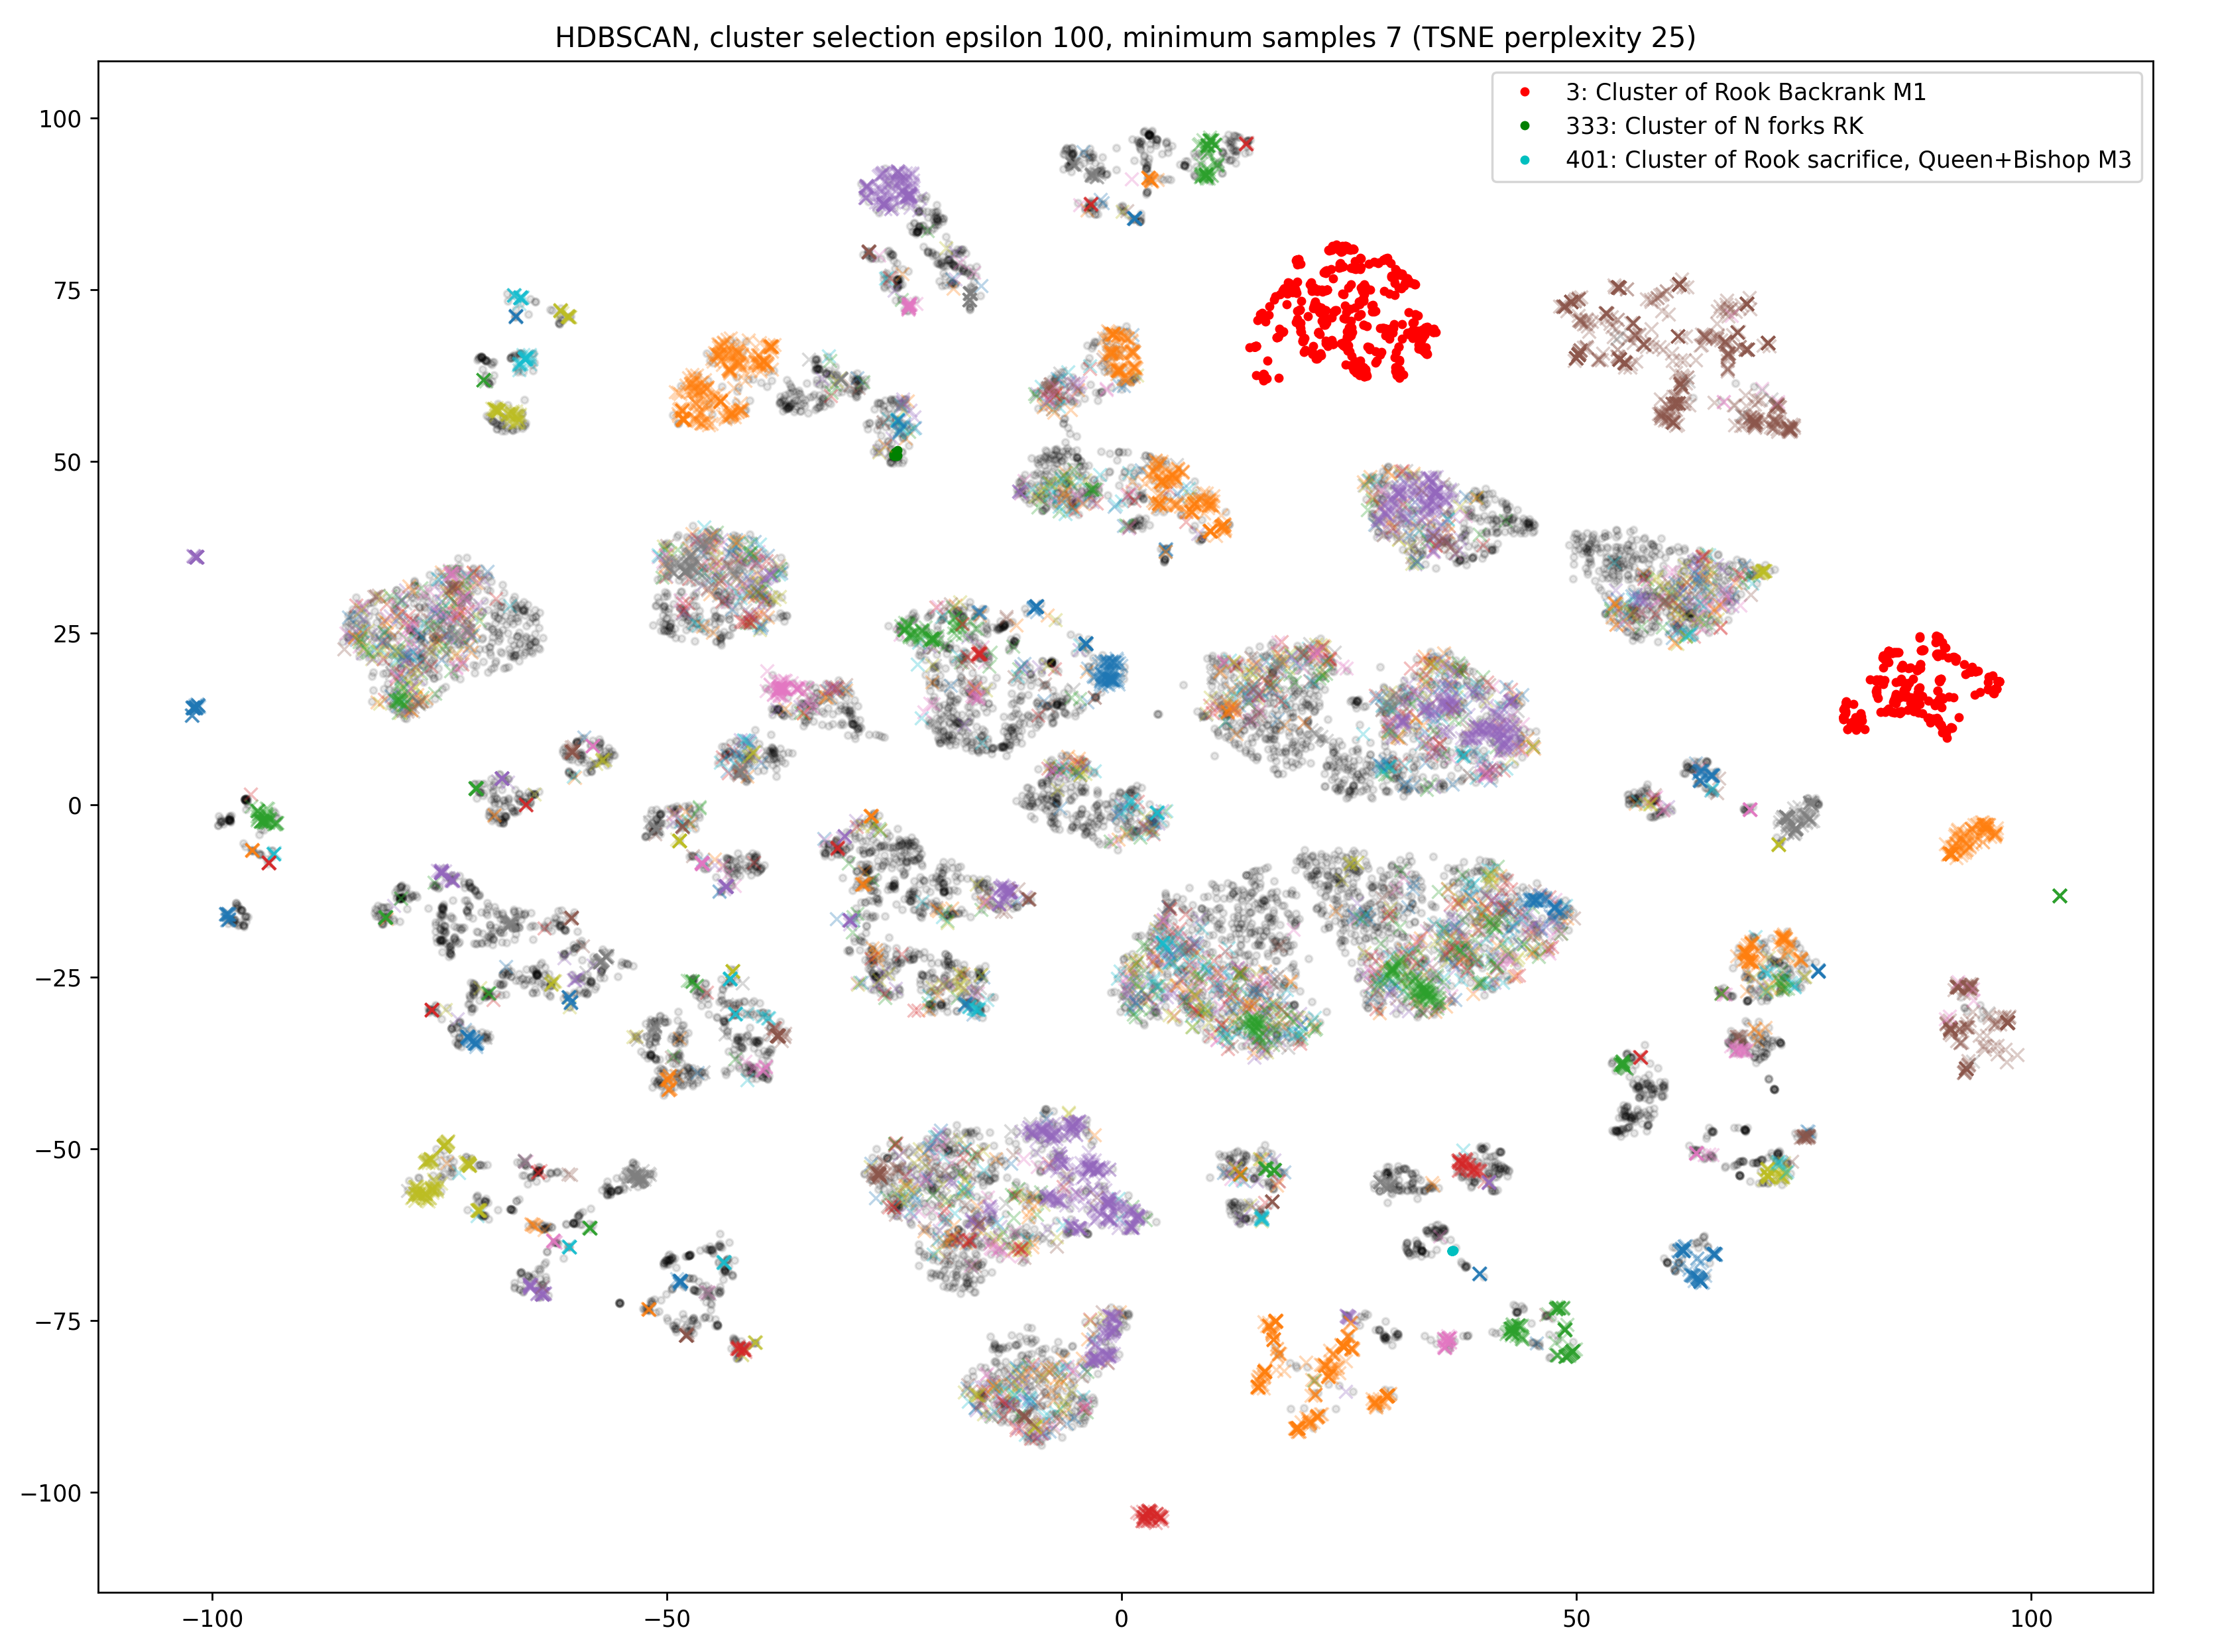
\includegraphics[width=\textwidth]{project/img/tsne/hdbscan_2_25.png}
  \caption{HDBSCAN, cluster selection $\epsilon=100$, minimum samples $7$.}
  \label{tsne3}
\end{figure}

\begin{figure}[H]
    \begin{minipage}{0.475\textwidth}
        \centering
        \chessboard[setfen=3r2r1/PR6/2pk2p1/1p1p1nP1/3PnPQ1/1PP1P3/2K5/5R2 b -
        - 0 39]
        \caption{Fork cluster puzzle. Black forks with \texttt{1...Nxe3+}}
        \label{hCl1}
    \end{minipage}
    \hspace{0.05\textwidth}
    \begin{minipage}{0.475\textwidth}
        \centering
        \chessboard[setfen=
        rn1q1b1r/pp3kpp/2p2n2/4p3/4p1b1/2NP1N2/PPP2PPP/R1BQK2R w KQ - 0 8]
        \caption{Fork cluster puzzle. White wins a bishop after
        \texttt{1.Nxe5+}}
        \label{hCl2}
    \end{minipage}
\end{figure}

Exploring clusters further, we observe that there exists a cluster of 61
puzzles, 56 of which are tagged as `endgame', a further 37 as `rook endgame',
and none are tagged with any sort of `mate'. This cluster appears to contain
various rook and pawn endgames, where the opposing side offers a rook trade.
Accepting the trade is the only winning move for the side solving the puzzle,
and this cluster encapsulates this. Figure \ref{chess15} contains an easy
puzzle from this cluster, and Figure \ref{chess16} contains a more complex
puzzle.

\begin{figure}[H]
    \begin{minipage}{0.475\textwidth}
        \centering
        \chessboard[setfen=8/8/k5r1/p5R1/5K2/P7/8/8 b - - 1 51]
        \caption{Rook trade cluster. After \texttt{1...Rxg5 2.Kxg5 Kb5}, Black
        wins the remaining pawn and shoulders the white king for a victory.}
        \label{chess15}
    \end{minipage}
    \hspace{0.05\textwidth}
    \begin{minipage}{0.475\textwidth}
        \centering
        \chessboard[setfen=8/2p4p/1k4p1/p1r5/2R4P/1P2K3/P4P2/8 b - - 3 47]
        \caption{Rook trade cluster. \texttt{1...Re5+} is tempting, and was
        played in the game where this position occured. This, however, loses
        the advantage. \texttt{1...Rxc4 2.bxc4} leads to a victory, despite the
        material balance.}
        \label{chess16}
    \end{minipage}
\end{figure}

